\documentclass[tikz,border=3pt]{standalone}
\usepackage{amsmath}
\usetikzlibrary{arrows.meta,positioning,calc,fit}
\definecolor{esrblue}{RGB}{34,91,151}
\definecolor{caporange}{RGB}{190,92,20}
\begin{document}
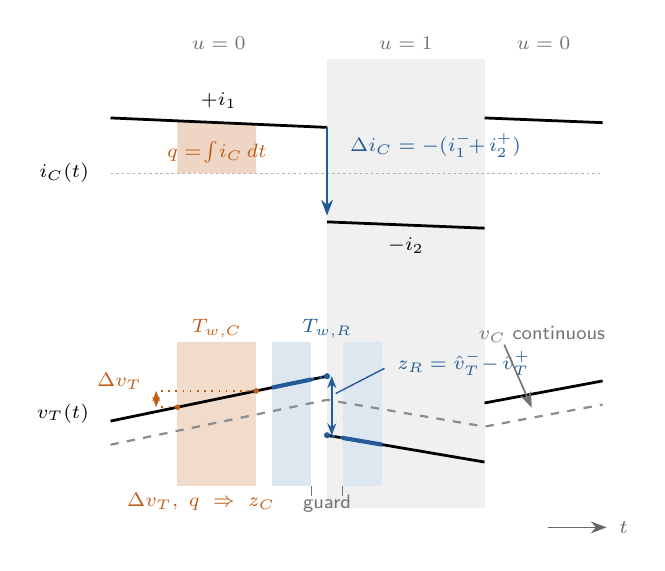
\begin{tikzpicture}[
  font=\sffamily\footnotesize,
  arr/.style={-{Stealth[length=2.0mm]},line width=0.8pt},
  wave/.style={line width=1.0pt},
  lbl/.style={font=\sffamily\scriptsize}]

% time layout (x in cm): OFF [0,2.75] | ON [2.75,4.75] | OFF [4.75,6.25]
% featured 0->1 edge at x=2.75; guard exaggerated for readability
% switch-state background bands + labels
\fill[black!6] (2.75,0.35) rectangle (4.75,6.05);
\node[lbl,black!55] at (1.375,6.25) {$u=0$};
\node[lbl,black!55] at (3.75,6.25) {$u=1$};
\node[lbl,black!55] at (5.5,6.25) {$u=0$};

% ---- iC(t) row ----
\node[lbl,anchor=east] at (-0.15,4.6) {$i_C(t)$};
\draw[black!30,dash pattern=on 1pt off 1pt] (0,4.6) -- (6.25,4.6);
% charge integral: area under the actual segment
\fill[caporange!25] (0.85,4.6) -- (1.85,4.6) -- (1.85,5.219)
  -- (0.85,5.263) -- cycle;
\draw[wave,black] (0,5.30) -- (2.75,5.18);
\draw[wave,black] (2.75,3.98) -- (4.75,3.90);
\draw[wave,black] (4.75,5.30) -- (6.25,5.24);
\node[lbl] at (1.375,5.52) {$+i_1$};
\node[lbl] at (3.75,3.68) {$-i_2$};
\draw[arr,esrblue] (2.75,5.18) -- (2.75,4.06);
\node[lbl,esrblue,anchor=west] at (2.92,4.95)
  {$\Delta i_C=-(i_1^-\!{+}\,i_2^+)$};
\node[lbl,caporange] at (1.35,4.86) {$q=\!\int\! i_C\,dt$};

% ---- vT(t) row ----
\node[lbl,anchor=east] at (-0.15,1.55) {$v_T(t)$};
% windows (guard = 0.20 visual)
\fill[caporange!22] (0.85,0.62) rectangle (1.85,2.45);
\fill[esrblue!15] (2.05,0.62) rectangle (2.55,2.45);
\fill[esrblue!15] (2.95,0.62) rectangle (3.45,2.45);
% vC dashed (continuous through the edge)
\draw[black!45,dashed,line width=0.8pt] (0,1.15) -- (2.75,1.72)
  -- (4.75,1.38) -- (6.25,1.66);
% vT solid with ESR discontinuities
\draw[wave,black] (0,1.45) -- (2.75,2.02);
\draw[wave,black] (2.75,1.27) -- (4.75,0.93);
\draw[wave,black] (4.75,1.68) -- (6.25,1.96);
% local fits inside the windows + dotted extrapolation to the edge time
\draw[esrblue,line width=1.5pt] (2.05,1.875) -- (2.55,1.979);
\draw[esrblue,dotted,line width=1.0pt] (2.55,1.979) -- (2.75,2.02);
\draw[esrblue,line width=1.5pt] (2.95,1.236) -- (3.45,1.151);
\draw[esrblue,dotted,line width=1.0pt] (2.95,1.236) -- (2.75,1.27);
\fill[esrblue] (2.75,2.02) circle (1.1pt);
\fill[esrblue] (2.75,1.27) circle (1.1pt);
\draw[{Stealth[length=1.5mm]}-{Stealth[length=1.5mm]},esrblue,line width=0.8pt]
  (2.81,2.02) -- (2.81,1.27);
\node[lbl,esrblue,anchor=west] at (3.52,2.18)
  {$z_R=\hat v_T^-{-}\,\hat v_T^+$};
\draw[esrblue,line width=0.5pt] (2.86,1.80) -- (3.48,2.12);
% charge-window endpoints on vT with left-side projection measurement
\fill[caporange] (0.85,1.626) circle (1.0pt);
\fill[caporange] (1.85,1.833) circle (1.0pt);
\draw[caporange,dotted,line width=0.6pt] (0.85,1.626) -- (0.58,1.626);
\draw[caporange,dotted,line width=0.6pt] (1.85,1.833) -- (0.58,1.833);
\draw[{Stealth[length=1.3mm]}-{Stealth[length=1.3mm]},caporange,
  line width=0.7pt] (0.58,1.626) -- (0.58,1.833);
\node[lbl,caporange,anchor=east] at (0.52,1.95) {$\Delta v_T$};
% labels
\node[lbl,esrblue] at (2.75,2.62) {$T_{w,R}$};
\node[lbl,caporange] at (1.35,2.62) {$T_{w,C}$};
\node[lbl,caporange] at (1.15,0.42) {$\Delta v_T,\ q\ \Rightarrow\ z_C$};
\node[lbl,black!55,anchor=west] at (4.55,2.55) {$v_C$ continuous};
\draw[arr,black!55,line width=0.6pt] (5.00,2.42) -- (5.35,1.62);
% guard ticks
\draw[black!55] (2.55,0.62) -- (2.55,0.50);
\draw[black!55] (2.95,0.62) -- (2.95,0.50);
\node[lbl,black!55] at (2.75,0.40) {guard};
% time arrow
\draw[arr,black!60,line width=0.6pt] (5.55,0.10) -- (6.30,0.10)
  node[lbl,black!60,right=1pt] {$t$};
\end{tikzpicture}
\end{document}
